\documentclass{article}
\usepackage[utf8]{inputenc}
\usepackage{amsfonts,amsthm,amsmath,amssymb,mathtools}
\usepackage{tikz}
\usetikzlibrary{arrows,backgrounds,matrix,positioning,shapes.geometric,
shapes.misc,calc,patterns}
\usepackage[]{xcolor}

\begin{document}

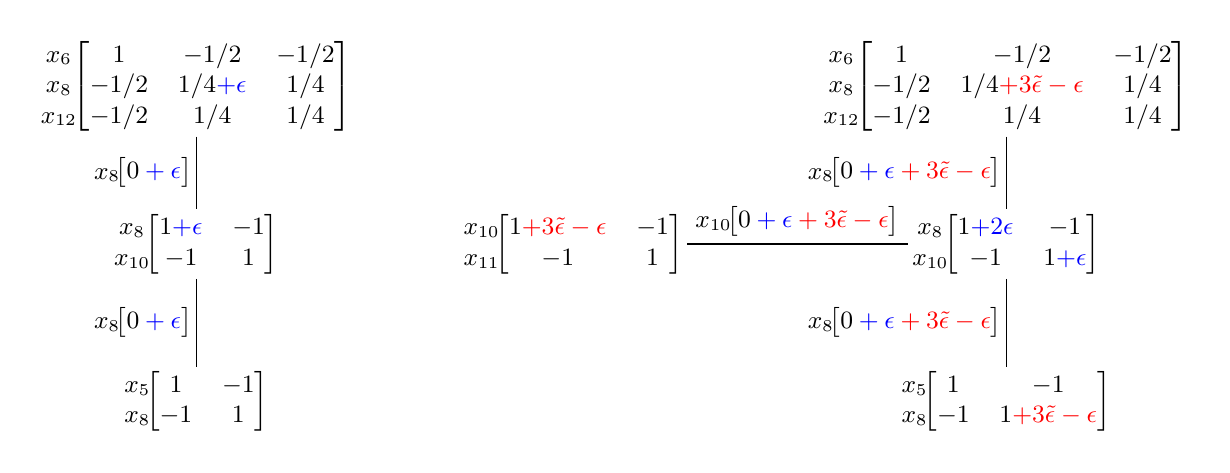
\begin{tikzpicture}
  \matrix ()[matrix of math nodes,
          column sep={5.5cm,between origins},
          row sep={2cm,between origins},
          nodes={font=\small,inner sep=.5mm}] at (8,0)
    { & |(c6)| \begin{matrix}x_6 \\ x_8 \\ x_{12}\end{matrix}\!\!
    \begin{bmatrix}1 &\hspace{-1em} -1/2 &\hspace{-1em} -1/2 \\ -1/2 &\hspace{-1em} 1/4{\color{red}+3\tilde{\epsilon}-\epsilon} &\hspace{-1em} 1/4 \\
    -1/2 &\hspace{-1em} 1/4 &\hspace{-1em} 1/4\end{bmatrix} \\
    |(c10)| \begin{matrix}x_{10} \\ x_{11}\end{matrix}\!\!
    \begin{bmatrix}1{\color{red}+3\tilde{\epsilon}-\epsilon} &\hspace{-1em} -1 \\ -1 &\hspace{-1em} 1\end{bmatrix} &
    |(c8)| \begin{matrix}x_8 \\ x_{10}\end{matrix}\!\!
    \begin{bmatrix}1\textcolor{blue}{+2\epsilon} &\hspace{-1em} -1 \\ -1 &\hspace{-1em} 1{\color{blue}+\epsilon}\end{bmatrix} \\
    & |(c5)| \begin{matrix}x_5 \\ x_8\end{matrix}\!\!
    \begin{bmatrix}1 &\hspace{-1em} -1 \\ -1 &\hspace{-1em} 1{\color{red}+3\tilde{\epsilon}-\epsilon}\end{bmatrix} \\};
  \matrix ()[matrix of math nodes,
          column sep={4cm,between origins},
          row sep={2cm,between origins},
          nodes={font=\small,inner sep=.5mm}] at (0,0)
    { |(c6_2)| \begin{matrix}x_6 \\ x_8 \\ x_{12}\end{matrix}\!\!
    \begin{bmatrix}1 &\hspace{-1em} -1/2 &\hspace{-1em} -1/2 \\ -1/2 &\hspace{-1em} 1/4{\color{blue}+\epsilon} &\hspace{-1em} 1/4 \\
    -1/2 &\hspace{-1em} 1/4 &\hspace{-1em} 1/4\end{bmatrix} \\
    |(c8_2)| \begin{matrix}x_8 \\ x_{10}\end{matrix}\!\!
    \begin{bmatrix}1{\color{blue}+\epsilon} &\hspace{-1em} -1 \\ -1 &\hspace{-1em} 1\end{bmatrix} \\
    |(c5_2)| \begin{matrix}x_5 \\ x_8\end{matrix}\!\!
    \begin{bmatrix}1 &\hspace{-1em} -1 \\ -1 &\hspace{-1em} 1\end{bmatrix} \\};
  \begin{scope}[every node/.style={font=\small,midway,inner sep=.5mm}]
    \draw (c10) -- node[above,yshift=.1em](){$x_{10}\!\!\begin{bmatrix}
      0\color{blue}+\epsilon\color{red}+3\tilde{\epsilon}-\epsilon\end{bmatrix}$}(c8);
    \draw (c8) -- node[left](){$x_8\!\!\begin{bmatrix}{0\color{blue}+\epsilon}\color{red}+3\tilde{\epsilon}-\epsilon\end{bmatrix}$}(c5);
    \draw (c6) -- node[left](){$x_8\!\!\begin{bmatrix}{0\color{blue}+\epsilon}\color{red}+3\tilde{\epsilon}-\epsilon\end{bmatrix}$}(c8);
    \draw (c8_2) -- node[left](){$x_8\!\!\begin{bmatrix}{0\color{blue}+\epsilon}\end{bmatrix}$}(c5_2);
    \draw (c6_2) -- node[left](){$x_8\!\!\begin{bmatrix}{0\color{blue}+\epsilon}\end{bmatrix}$}(c8_2);
  \end{scope}
\end{tikzpicture}

\end{document}